\begin{frame}{Missing value imputation}

\begin{itemize}
    \item Data can be missing in different ways:
    \begin{itemize}
        \item Missing Completely at Random (MCAR): purely random points are missing
        \item Missing at Random (MAR): something affects missingness, but no relation with the value
        \begin{itemize}
            \item E.g. faulty sensors, some people don't fill out forms correctly
        \end{itemize}
        \item Missing Not At Random (MNAR): systematic missingness linked to the value
        \begin{itemize}
            \item Has to be modelled or resolved (e.g. sensor decay, sick people leaving study)
        \end{itemize}
    \end{itemize}

    \item Missingness can be encoded in different ways: \texttt{'?'}, \texttt{'-1'}, \texttt{'unknown'}, \texttt{'NA'},\ldots

    \item Also labels can be missing (remove example or use semi-supervised learning)
\end{itemize}

\end{frame}


\begin{frame}{Overview}

\begin{itemize}
    \item Mean/constant imputation
    \item kNN-based imputation
    \item Iterative (model-based) imputation
    \item Matrix Factorization techniques
\end{itemize}

\vspace{1em}

\begin{center}
    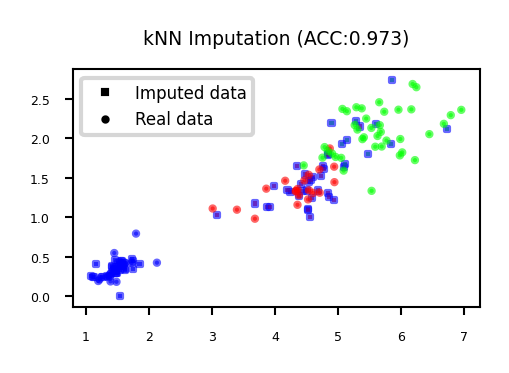
\includegraphics[width=0.6\textwidth]{images/pre-processing/knn-imputation.png}
\end{center}

\end{frame}


\begin{frame}[allowframebreaks]{Mean imputation}

\begin{itemize}
    \item Replace all missing values of a feature by the same value
    \begin{itemize}
        \item Numerical features: mean or median
        \item Categorical features: most frequent category
        \item Constant value, e.g. 0 or \texttt{'missing'} for text features
    \end{itemize}

    \item Optional: add an indicator column for missingness

    \item Example: Iris dataset (randomly removed values in 3rd and 4th column)
\end{itemize}

\vspace{1em}

\begin{center}
    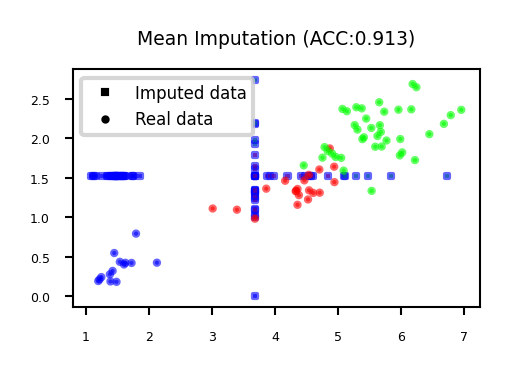
\includegraphics[width=0.6\textwidth]{images/pre-processing/mean-imputation.png}
\end{center}

\end{frame}


\begin{frame}{kNN imputation}

\begin{itemize}
    \item Use special version of kNN to predict value of missing points
    \item Uses only non-missing data when computing distances
\end{itemize}

\vspace{1em}

\begin{center}
    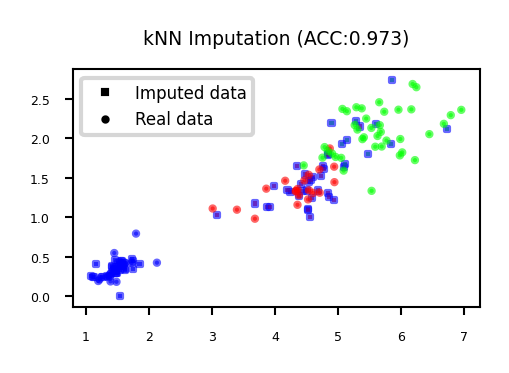
\includegraphics[width=0.6\textwidth]{images/pre-processing/knn-imputation.png}
\end{center}

\end{frame}


\begin{frame}[allowframebreaks]{Iterative (model-based) Imputation}

\begin{itemize}
    \item Better known as Multiple Imputation by Chained Equations (MICE)
    \item Iterative approach
    \begin{itemize}
        \item Do first imputation (e.g. mean imputation)
        \item Train model (e.g. RandomForest) to predict missing values of a given feature
        \item Train new model on imputed data to predict missing values of the next feature
        \begin{itemize}
            \item Repeat $m$ times in round-robin fashion, leave one feature out at a time
        \end{itemize}
    \end{itemize}
\end{itemize}

\vspace{1em}

\begin{center}
    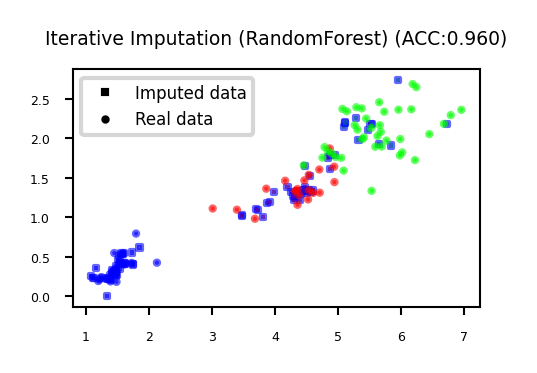
\includegraphics[width=0.6\textwidth]{images/pre-processing/iterative-imputation.png}
\end{center}

\end{frame}


\begin{frame}[allowframebreaks]{Matrix Factorization}

\begin{itemize}
    \item Basic idea: low-rank approximation
    \begin{itemize}
        \item Replace missing values by 0
        \item Factorize $\mathbf{X}$ with rank $r$: 
        $\mathbf{X}^{n \times p} = \mathbf{U}^{n \times r} \mathbf{V}^{r \times p}$
        \begin{itemize}
            \item With $n$ data points and $p$ features
            \item Solved using gradient descent
        \end{itemize}
        \item Recompute $\mathbf{X}$: now complete
    \end{itemize}
\end{itemize}

\vspace{1em}

\begin{center}
    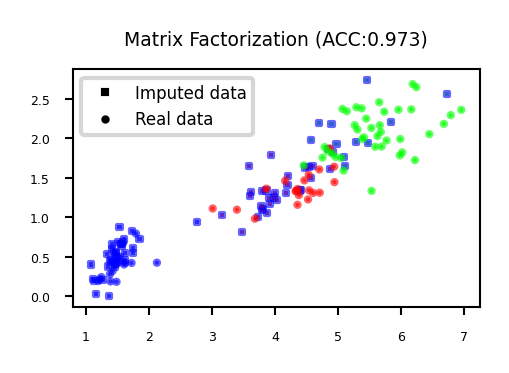
\includegraphics[width=0.6\textwidth]{images/pre-processing/matrix-factorization.png}
\end{center}

\end{frame}


\begin{frame}[allowframebreaks]{Soft-thresholded Singular Value Decomposition (SVD)}

\begin{itemize}
    \item Same basic idea, but smoother
    \begin{itemize}
        \item Replace missing values by 0, compute SVD: $\mathbf{X} = \mathbf{U} \mathbf{\Sigma} \mathbf{V}^\top$
        \begin{itemize}
            \item Solved with gradient descent
        \end{itemize}
        \item Reduce eigenvalues by shrinkage factor: $\lambda_i = s \cdot \lambda_i$
        \item Recompute $\mathbf{X}$: now complete
        \item Repeat for $m$ iterations
    \end{itemize}
\end{itemize}

\vspace{1em}

\begin{center}
    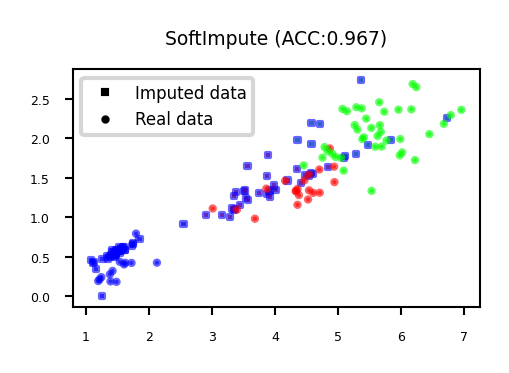
\includegraphics[width=0.6\textwidth]{images/pre-processing/softimpute.png}
\end{center}

\end{frame}


\begin{frame}{Comparison}

\begin{itemize}
    \item Best method depends on the problem and dataset at hand. Use cross-validation.
    \item Iterative Imputation (MICE) generally works well for missing (completely) at random data
    \begin{itemize}
        \item Can be slow if the prediction model is slow
    \end{itemize}
    \item Low-rank approximation techniques scale well to large datasets
\end{itemize}

\vspace{1em}

\begin{center}
    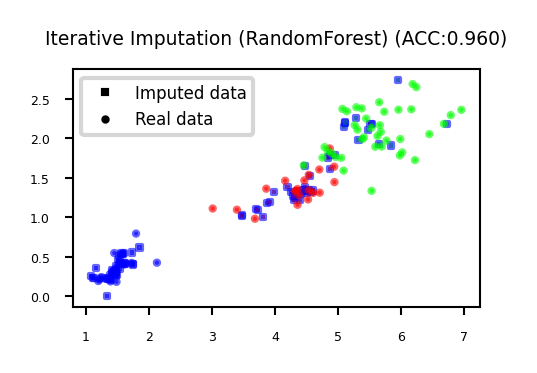
\includegraphics[width=0.6\textwidth]{images/pre-processing/iterative-imputation.png}
\end{center}

\end{frame}


% \begin{frame}[fragile,allowframebreaks]{In practice (scikit-learn)}
% \scriptsize
% \begin{itemize}
%     \item Simple replacement: \texttt{SimpleImputer}
%     \begin{itemize}
%         \item Strategies: \texttt{mean} (numeric), \texttt{median}, \texttt{most\_frequent} (categorical)
%         \item Choose whether to add indicator columns, and how missing values are encoded
%     \end{itemize}
% \end{itemize}

% \begin{verbatim}
% imp = SimpleImputer(strategy='mean', missing_values=np.nan,
%                     add_indicator=False)
% X_complete = imp.fit_transform(X_train)
% \end{verbatim}

% \begin{itemize}
%     \item kNN Imputation: \texttt{KNNImputer}
% \end{itemize}

% \begin{verbatim}
% imp = KNNImputer(n_neighbors=5)
% X_complete = imp.fit_transform(X_train)
% \end{verbatim}

% \begin{itemize}
%     \item Multiple Imputation (MICE): \texttt{IterativeImputer}
%     \begin{itemize}
%         \item Choose estimator (default: \texttt{BayesianRidge}) and number of iterations (default 10)
%     \end{itemize}
% \end{itemize}

% \begin{verbatim}
% imp = IterativeImputer(estimator=RandomForestClassifier(), max_iter=10)
% X_complete = imp.fit_transform(X_train)
% \end{verbatim}
% \end{frame}


% \begin{frame}[fragile,allowframebreaks]{In practice (fancyimpute)}
% \scriptsize
% \begin{itemize}
%     \item Cannot be used in CV pipelines (has \texttt{fit\_transform} but no \texttt{transform})
    
%     \item Soft-Thresholded SVD: \texttt{SoftImpute}
%     \begin{itemize}
%         \item Choose max number of gradient descent iterations
%         \item Choose shrinkage value for eigenvectors (default: $\frac{1}{N}$)
%     \end{itemize}
% \end{itemize}

% \begin{verbatim}
% imp = SoftImpute(max_iter=10, shrinkage_value=None)
% X_complete = imp.fit_transform(X)
% \end{verbatim}

% \begin{itemize}
%     \item Low-rank imputation: \texttt{MatrixFactorization}
%     \begin{itemize}
%         \item Choose rank of the low-rank approximation
%         \item Gradient descent hyperparameters: learning rate, epochs, ...
%         \item Several variants exist
%     \end{itemize}
% \end{itemize}

% \begin{verbatim}
% imp = MatrixFactorization(rank=10, learning_rate=0.001, epochs=10000)
% X_complete = imp.fit_transform(X)
% \end{verbatim}
% \end{frame}

